\documentclass[a4paper,12pt]{article}

\usepackage{cite}
\usepackage{amsmath,amssymb,amsfonts}
\usepackage{algorithmic}
\usepackage{graphicx}
\usepackage{textcomp}
\usepackage{xcolor}
\usepackage{booktabs}
\usepackage{url}
\def\BibTeX{{\rm B\kern-.05em{\sc i\kern-.025em b}\kern-.08em
    T\kern-.1667em\lower.7ex\hbox{E}\kern-.125emX}}
\begin{document}

\title{Assignment 2 : Anomaly Detection %\\
%{\footnotesize \textsuperscript{*}Note: Sub-titles are not captured for https://ieeexplore.ieee.org  and
%should not be used}
%\thanks{Identify applicable funding agency here. If none, delete this.}
}

\author{Renjiro Owen\\
\textit{Victoria University Wellington}\\
Wellington, New Zealand\\
owenrenj@myvuw.ac.nz}

\maketitle
\newpage
\section{Preprocessing the Data}
The \textit{year} variable was removed because it does not provide meaningful information for the clustering analysis and may introduce unnecessary variation between the two years. The \textit{day of year} variable was transformed using sine and cosine functions to represent its cyclical nature, where the end of one year is close to the beginning of the next. This transformation preserves the continuous progression of days and avoids treating the first and last days of the year as being far apart. For the nominal \textit{season} variable, sine and cosine transformations were also used to represent the cyclical relationship between seasons. This allows adjacent seasons to have similar representations while also capturing the contrasting relationship between opposite seasons, such as summer and winter, without treating the season categories as independent numerical values. The resulting transformed features can be seen in Figure~\ref{fig:preprocess}.
\begin{figure}
	\centering
	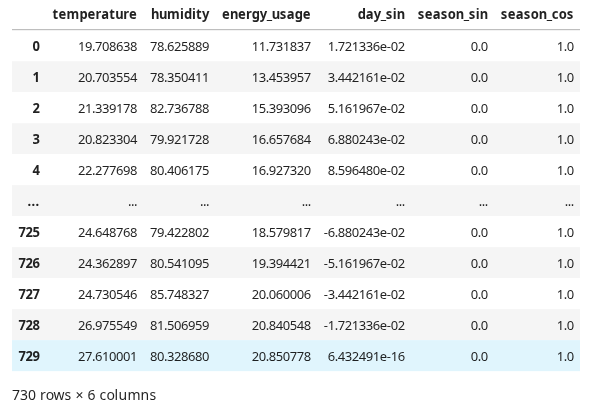
\includegraphics[width=0.8\textwidth]{../../preprocess.png}
	\caption{K-means clustering with $K=3$.}
	\label{fig:preprocess}
\end{figure}

\section{Experimenting with Isolation Forest and LOF}
\begin{table}
	\centering
	\caption{Isolation Forest and Local Outlier Factor Performance.}
	\label{tab:if_lof}
	\scriptsize
	\begin{tabular}{lcccccc}
		\hline
		Model & Recall & Precision & F1 & Correct & Missed & False Positives \\
		\hline
		Isolation Forest & 0.833 & 0.070 & 0.129 & 15 & 3 & 200 \\
		Local Outlier Factor & 0.444 & 0.267 & 0.333 & 8 & 10 & 22 \\
		\hline
	\end{tabular}
\end{table}

Table~\ref{tab:if_lof} shows that Isolation Forest (IF) achieved a higher recall of 0.833 compared with 0.444 for Local Outlier Factor (LOF), meaning that IF detected a larger proportion of the actual anomalies. However, LOF achieved substantially higher precision (0.267 compared with 0.070) and a higher F1 score (0.333 compared with 0.129), indicating that its predictions contained fewer false positives. This difference is also reflected in the number of false positives, with IF producing 200 compared with only 22 for LOF, while IF correctly identified more anomalies (15 compared with 8).

These results reflect the different ways the two algorithms identify anomalies. Isolation Forest identifies observations that are easier to isolate from the rest of the data, allowing it to detect more potential anomalies but also causing it to classify many normal observations as anomalies. In contrast, LOF considers the local density of observations and identifies points that have substantially lower density than their surrounding neighbourhood, resulting in fewer false positives but also causing it to miss more anomalies. Therefore, IF would be preferable when detecting as many potential anomalies as possible is the priority and false positives can be investigated afterwards, whereas LOF would be more suitable when precision is more important and false alarms are costly.

\section{Hyperparameter Tuning}
\subsection{Parameter Tune}

F1 score was used as the primary metric for selecting the better model configuration because it provides a balance between precision and recall. From the initial experiments, contamination values of 0.03 and 0.05 were identified as the most promising settings, achieving F1 scores of 0.250 and 0.255, respectively. Therefore, these two contamination values were selected for further hyperparameter tuning of Isolation Forest (IF) and Local Outlier Factor (LOF). The results of the initial contamination experiments are shown in Table~\ref{tab:contamination}.

\begin{table}
	\centering
	\small
	\setlength{\tabcolsep}{5pt}
	\caption{Performance of different contamination values.}
	\label{tab:contamination}
	\begin{tabular}{lcccccc}
		\hline
		Contamination & Recall & Precision & F1 & Correct & Missed & FP \\
		\hline
		0.01 & 0.111 & 0.250 & 0.154 & 2 & 16 & 6 \\
		0.03 & 0.278 & 0.227 & 0.250 & 5 & 13 & 17 \\
		0.05 & 0.389 & 0.189 & 0.255 & 7 & 11 & 30 \\
		0.10 & 0.556 & 0.137 & 0.220 & 10 & 8 & 63 \\
		0.15 & 0.667 & 0.109 & 0.188 & 12 & 6 & 98 \\
		0.20 & 0.722 & 0.089 & 0.159 & 13 & 5 & 133 \\
		0.25 & 0.833 & 0.082 & 0.149 & 15 & 3 & 168 \\
		0.30 & 0.833 & 0.068 & 0.127 & 15 & 3 & 204 \\
		0.35 & 0.889 & 0.062 & 0.117 & 16 & 2 & 240 \\
		0.40 & 0.889 & 0.055 & 0.103 & 16 & 2 & 276 \\
		0.45 & 1.000 & 0.055 & 0.104 & 18 & 0 & 311 \\
		0.50 & 1.000 & 0.049 & 0.094 & 18 & 0 & 347 \\
		\hline
	\end{tabular}
\end{table}

\subsection{Isolation Forest}

For Isolation Forest, the number of estimators was varied from 100 to 500 for the two selected contamination values. At a contamination value of 0.03, the best F1 score was 0.250, obtained with 100 and 400 estimators. Increasing the number of estimators to 200, 300, or 500 resulted in a lower F1 score of 0.200. At a contamination value of 0.05, the best performance was achieved with 200--500 estimators, all producing a recall of 0.500, precision of 0.243, and F1 score of 0.327. Therefore, the best IF configuration was contamination =0.05 with n\_estimators=200, as it achieved the highest F1 score of 0.327.

\begin{table}
	\centering
	\small
	\setlength{\tabcolsep}{5pt}
	\caption{Isolation Forest parameter tuning results.}
	\label{tab:if_tuning}
	\begin{tabular}{llcccccc}
		\hline
		Cont. & $n_{\mathrm{est}}$ & Recall & Precision & F1 & Correct & Missed & FP \\
		\hline
		0.03 & 100 & 0.278 & 0.227 & 0.250 & 5 & 13 & 17 \\
		0.03 & 200 & 0.222 & 0.182 & 0.200 & 4 & 14 & 18 \\
		0.03 & 300 & 0.222 & 0.182 & 0.200 & 4 & 14 & 18 \\
		0.03 & 400 & 0.278 & 0.227 & 0.250 & 5 & 13 & 17 \\
		0.03 & 500 & 0.222 & 0.182 & 0.200 & 4 & 14 & 18 \\
		0.05 & 100 & 0.389 & 0.189 & 0.255 & 7 & 11 & 30 \\
		0.05 & 200 & 0.500 & 0.243 & 0.327 & 9 & 9 & 28 \\
		0.05 & 300 & 0.500 & 0.243 & 0.327 & 9 & 9 & 28 \\
		0.05 & 400 & 0.500 & 0.243 & 0.327 & 9 & 9 & 28 \\The selection was based on a
		0.05 & 500 & 0.500 & 0.243 & 0.327 & 9 & 9 & 28 \\
		\hline
	\end{tabular}
\end{table}

\subsection{Local Outlier Factor}

For LOF, the number of neighbours was varied from 5 to 70 using the same two contamination values. With contamination=0.03, the highest F1 score of 0.500 was obtained with n\_neighbors=5, while larger neighbourhood sizes generally reduced the F1 score. With contamination=0.05, the highest F1 score was 0.400, also achieved with n\_neighbors=5. Therefore, the best LOF configuration was contamination=0.03 with n\_neighbors=5, achieving a recall of 0.556, precision of 0.455, and F1 score of 0.500.

\begin{table}
	\centering
	\small
	\setlength{\tabcolsep}{5pt}
	\caption{Local Outlier Factor parameter tuning results.}
	\label{tab:lof_tuning}
	\begin{tabular}{llcccccc}
		\hline
		Cont. & $n_{\mathrm{neigh}}$ & Recall & Precision & F1 & Correct & Missed & FP \\
		\hline
		0.03 & 5  & 0.556 & 0.455 & 0.500 & 10 & 8 & 12 \\
		0.03 & 10 & 0.444 & 0.364 & 0.400 & 8 & 10 & 14 \\
		0.03 & 20 & 0.333 & 0.273 & 0.300 & 6 & 12 & 16 \\
		0.03 & 30 & 0.278 & 0.227 & 0.250 & 5 & 13 & 17 \\
		0.03 & 40 & 0.278 & 0.227 & 0.250 & 5 & 13 & 17 \\
		0.03 & 50 & 0.389 & 0.318 & 0.350 & 7 & 11 & 15 \\
		0.03 & 60 & 0.389 & 0.318 & 0.350 & 7 & 11 & 15 \\
		0.03 & 70 & 0.333 & 0.273 & 0.300 & 6 & 12 & 16 \\
		0.05 & 5  & 0.611 & 0.297 & 0.400 & 11 & 7 & 26 \\
		0.05 & 10 & 0.500 & 0.243 & 0.327 & 9 & 9 & 28 \\
		0.05 & 20 & 0.444 & 0.216 & 0.291 & 8 & 10 & 29 \\
		0.05 & 30 & 0.444 & 0.216 & 0.291 & 8 & 10 & 29 \\
		0.05 & 40 & 0.556 & 0.270 & 0.364 & 10 & 8 & 27 \\
		0.05 & 50 & 0.444 & 0.216 & 0.291 & 8 & 10 & 29 \\
		0.05 & 60 & 0.444 & 0.216 & 0.291 & 8 & 10 & 29 \\
		0.05 & 70 & 0.444 & 0.216 & 0.291 & 8 & 10 & 29 \\
		\hline
	\end{tabular}
\end{table}

In terms of recall and precision, the tuning results show a clear trade-off between detecting more anomalies and reducing false positives. The best LOF configuration achieved the highest balance, with a recall of 0.556 and precision of 0.455, while the best IF configuration achieved a lower recall of 0.500 and precision of 0.243. Although LOF did not achieve the highest recall across all tested configurations, its substantially higher precision indicates that a greater proportion of its predicted anomalies were actually anomalous.

Overall, hyperparameter tuning improved the performance of both methods when compared with their initial configurations. The best IF configuration achieved an F1 score of 0.327, while the best LOF configuration achieved an F1 score of 0.500. Therefore, based on F1 score, LOF with contamination=0.03 and n\_neighbors=5 was the best-performing configuration among the tested models. This configuration also produced considerably fewer false positives than the initial Isolation Forest result, making it a more balanced choice for this dataset.

\section{Model Selection and Analysis}
F1 score was used as the primary metric for selecting the better model configuration because it provides a balance between precision and recall. The Local Outlier Factor (LOF) model with contamination=0.03 and n\_neighbors=5 was selected as the best model because it achieved the highest F1 score of 0.500 among the tested configurations. The selection was therefore based on a trade-off between recall and precision rather than optimising either metric independently. Although some configurations achieved higher recall, they also produced substantially more false positives, whereas the selected LOF configuration achieved a relatively high recall of 0.556 while maintaining a much higher precision of 0.455. Therefore, LOF was preferred because it provided the most balanced performance between detecting anomalies and avoiding incorrect anomaly classifications.

\subsection*{Analysis}
\begin{figure}
	\centering
	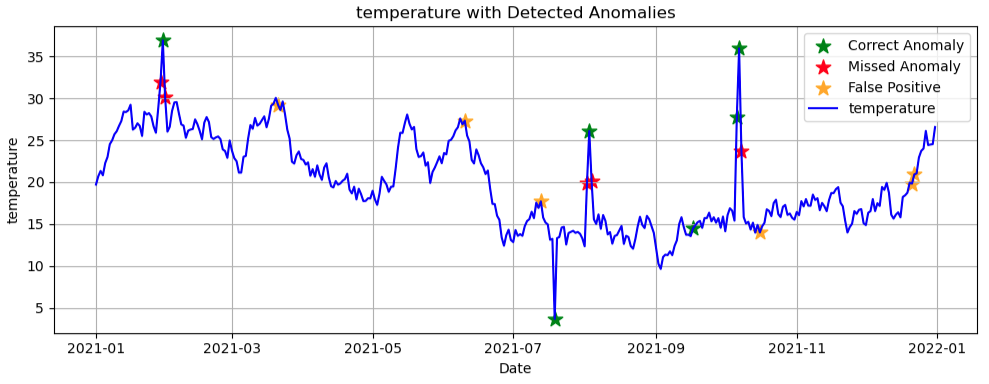
\includegraphics[width=0.8\textwidth]{../../tempLOFor.png}
	\caption{Temperature with Anomaly Detection.}
	\label{fig:temp}
\end{figure}
\begin{figure}
	\centering
	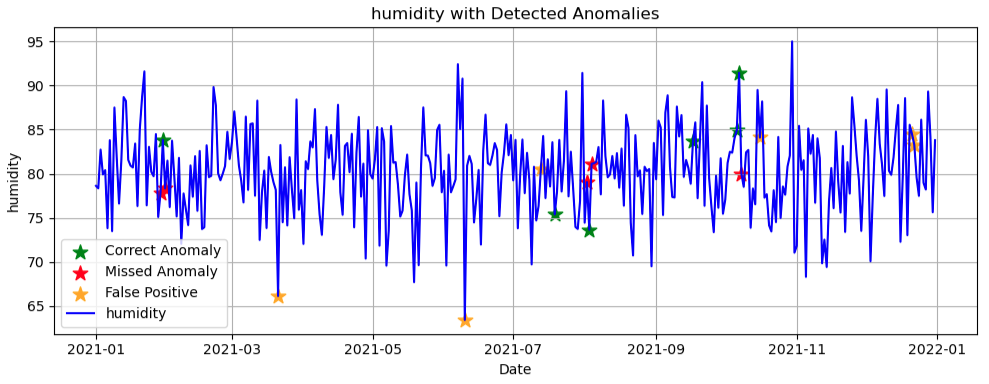
\includegraphics[width=0.8\textwidth]{../../humLOFor.png}
	\caption{Humidity with Anomaly Detection.}
	\label{fig:humidity}
\end{figure}
\begin{figure}
	\centering
	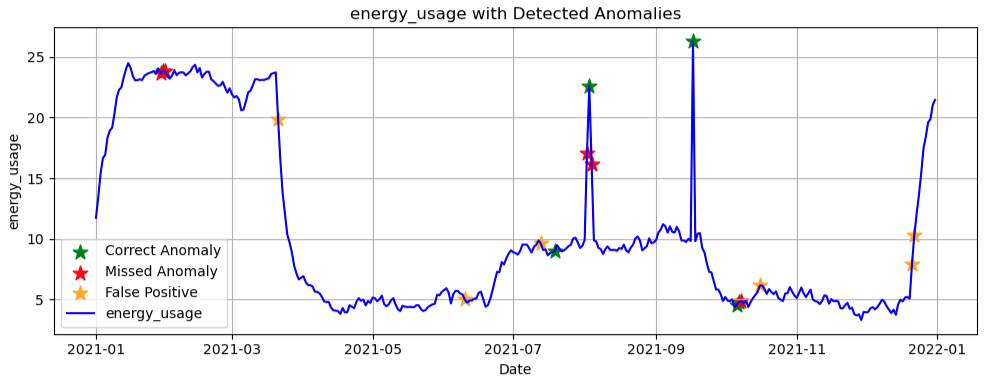
\includegraphics[width=0.8\textwidth]{../../eneLOFor.png}
	\caption{Energy Usage with Anomaly Detection.}
	\label{fig:energy_usage}
\end{figure}
The selected LOF model achieved a recall of 0.556, a precision of 0.455, and an F1 score of 0.500, correctly identifying 10 anomalies while missing 8 and producing 12 false positives. The detected and missed anomalies were analysed using the temperature, humidity, and energy usage patterns shown in Figures~\ref{fig:temp}, \ref{fig:humidity}, and \ref{fig:energy_usage}.

Between January and March, three anomalies can be observed in the temperature pattern. The middle observation has the highest temperature and was successfully detected by LOF, while the anomalies on either side were missed. This suggests that the two missed anomalies were less distinct from their local neighbourhoods and therefore did not have a sufficiently low local density to be classified as anomalies.

Between March and May, several false positives were identified. Although these observations did not appear to be extreme based on temperature, their humidity values were among the lowest in the dataset, as shown in Figure~\ref{fig:humidity}, while energy usage also appeared to shift towards lower values in Figure~\ref{fig:energy_usage}. This suggests that LOF detected these observations based on their local behaviour across multiple features rather than because of an extreme value in temperature alone. A similar pattern was observed for some of the false positives between May and July.

Around July and September, sudden increases in temperature and energy usage can be observed in Figures~\ref{fig:temp} and \ref{fig:energy_usage}, while the surrounding observations remained relatively low. Although these temperature values were not globally extreme and could be considered normal during summer, their occurrence during winter made them unusual in context. Therefore, these observations can be considered contextual anomalies. LOF successfully detected these anomalies, suggesting that it was able to identify unusual observations based on their local relationship with the surrounding data and seasonal conditions.

Finally, an increase in energy usage was observed towards December, where LOF produced a false positive as both energy usage and temperature increased rapidly. This observation was not necessarily a global anomaly, but the rapid change may have caused it to differ from its local neighbourhood and therefore receive a high LOF anomaly score. This demonstrates a potential limitation of LOF when dealing with changing seasonal or temporal patterns, as normal transitions in the data may appear anomalous when compared with nearby observations. Overall, the results show that LOF was able to detect both globally unusual observations and contextual anomalies, but it could miss anomalies that were not sufficiently different from their local neighbourhood or incorrectly flag normal changes in behaviour as anomalies.

\section{Exploration}

\subsection{Humidity Removal}

Based on the previous anomaly analysis, several false positives appeared to be associated with unusually high or low humidity values. Since some of these observations did not show similarly unusual temperature or energy usage, humidity may have contributed to incorrect anomaly classifications. Therefore, an alternative feature set excluding humidity was investigated. The LOF model was retrained using temperature, energy usage, and the temporal and seasonal features to determine whether removing humidity could reduce false positives and improve the overall anomaly detection performance.

\begin{table}
	\centering
	\small
	\setlength{\tabcolsep}{5pt}
	\caption{Performance after removing humidity.}
	\label{tab:humidity_removal}
	\begin{tabular}{lcccccc}
		\hline
		Model & Recall & Precision & F1 & Correct & Missed & FP \\
		\hline
		LOF & 0.722 & 0.591 & 0.650 & 13 & 5 & 9 \\
		IF & 0.611 & 0.297 & 0.400 & 11 & 7 & 26 \\
		\hline
	\end{tabular}
\end{table}

The results show that removing humidity substantially improved the performance of both methods, with LOF achieving a recall of 0.722, precision of 0.591, and F1 score of 0.650. Compared with the previous LOF result of 0.500 F1, the new feature set improved both recall and precision while reducing false positives from 12 to 9. Isolation Forest also achieved a higher recall of 0.611 and F1 score of 0.400 compared with its previous performance, although it still produced 26 false positives. These results suggest that humidity was introducing noise into the anomaly detection process and causing some normal observations with unusual humidity values to be incorrectly classified as anomalies. Therefore, removing humidity was effective for this dataset, and the improved LOF performance suggests that temperature, energy usage, and temporal/seasonal features provide more useful information for distinguishing the anomalies in the data.

\subsection{Temperature and Energy Usage Scaled}

After removing humidity, the remaining numerical features were further standardized to investigate whether differences in feature scales were affecting the anomaly detection results. In particular, temperature and energy usage were scaled so that features with larger numerical ranges would not disproportionately influence the distance- and density-based calculations used by LOF. The results are shown below.

\begin{table}
	\centering
	\small
	\setlength{\tabcolsep}{5pt}
	\caption{Performance after scaling temperature and energy usage.}
	\label{tab:scaled_results}
	\begin{tabular}{lcccccc}
		\hline
		Model & Recall & Precision & F1 & Correct & Missed & FP \\
		\hline
		LOF & 0.889 & 0.727 & 0.800 & 16 & 2 & 6 \\
		IF & 0.611 & 0.297 & 0.400 & 11 & 7 & 26 \\
		\hline
	\end{tabular}
\end{table}

The results show a substantial improvement in LOF performance after scaling, with recall increasing to 0.889, precision to 0.727, and F1 to 0.800. LOF correctly detected 16 of the 18 anomalies while missing only 2 and producing 6 false positives. Compared with the previous LOF result after humidity removal, the F1 score increased from 0.650 to 0.800, while the number of false positives decreased from 9 to 6. In contrast, the Isolation Forest results remained unchanged, indicating that scaling did not affect its performance in this experiment. This is expected because Isolation Forest is based on randomly selecting features and split values rather than calculating distances between observations. Overall, the results demonstrate that scaling was particularly beneficial for LOF because its local-density calculations are sensitive to the relative scale of the input features.

\subsection{AND Ensemble}

An AND-based ensemble was also investigated, where an observation was classified as an anomaly only when both Isolation Forest and LOF identified it as anomalous. The motivation for this approach was that requiring agreement between two different anomaly detection methods could provide greater confidence in the detected anomalies and reduce false alarms. The results are shown in Table~\ref{tab:ensemble_and}.

\begin{table}
	\centering
	\small
	\setlength{\tabcolsep}{5pt}
	\caption{Performance of the AND-based ensemble.}
	\label{tab:ensemble_and}
	\begin{tabular}{lcccccc}
		\hline
		Model & Recall & Precision & F1 & Correct & Missed & FP \\
		\hline
		Ensemble AND & 0.611 & 0.846 & 0.710 & 11 & 7 & 2 \\
		\hline
	\end{tabular}
\end{table}

The AND-based ensemble substantially reduced the number of false positives from 6 to 2 and increased precision from 0.727 to 0.846 compared with the tuned LOF model. However, recall decreased from 0.889 to 0.611 because several anomalies detected by LOF were not simultaneously detected by Isolation Forest. Consequently, the F1 score decreased from 0.800 to 0.710. This indicates that requiring agreement between both models produces a more conservative anomaly detector, improving precision at the cost of recall. Therefore, although the AND ensemble is useful when false positives are particularly costly, the individual LOF model remains preferable for this dataset because it achieves a higher F1 score and detects more of the actual anomalies.

\subsection{One-Class SVM}

One-Class SVM was investigated as an alternative anomaly detection method to determine whether a boundary-based approach could identify anomalies more effectively than Isolation Forest and LOF. Unlike LOF, which evaluates the local density of observations, One-Class SVM learns a boundary around the majority of the data and identifies observations that fall outside this learned boundary as anomalies. This approach was tested to determine whether the anomalies in the dataset could be separated effectively based on the overall structure of the preprocessed features.

\begin{table}
	\centering
	\small
	\setlength{\tabcolsep}{5pt}
	\caption{Performance of One-Class SVM.}
	\label{tab:ocsvm}
	\begin{tabular}{lcccccc}
		\hline
		Model & Recall & Precision & F1 & Correct & Missed & FP \\
		\hline
		One-Class SVM & 0.611 & 0.500 & 0.550 & 11 & 7 & 11 \\
		\hline
	\end{tabular}
\end{table}

One-Class SVM achieved a recall of 0.611, precision of 0.500, and F1 score of 0.550, correctly detecting 11 anomalies while missing 7 and producing 11 false positives. Although the model was able to detect more than half of the actual anomalies, its F1 score was lower than the tuned LOF model 0.800 and the AND ensemble 0.710. This suggests that the anomalies in this dataset are not separated from normal observations by a single clear global boundary, making the boundary-based approach of One-Class SVM less effective than the local-density approach of LOF. Therefore, One-Class SVM provided a reasonable alternative but did not improve upon the selected LOF model for this dataset.

\subsection{Vote Ensemble}

A voting-based ensemble was investigated to determine whether combining the predictions of multiple anomaly detection models could provide a better balance between detecting anomalies and avoiding false positives. Instead of requiring all models to agree, the observation was classified according to the majority vote of the models. This approach was motivated by the different behaviours of IF, LOF, and One-Class SVM, where each method may identify different types of anomalies.

\begin{table}
	\centering
	\small
	\setlength{\tabcolsep}{5pt}
	\caption{Performance of the voting-based ensemble.}
	\label{tab:ensemble_vote}
	\begin{tabular}{lcccccc}
		\hline
		Model & Recall & Precision & F1 & Correct & Missed & FP \\
		\hline
		Ensemble Vote & 0.778 & 0.737 & 0.757 & 14 & 4 & 5 \\
		\hline
	\end{tabular}
\end{table}

The voting ensemble achieved a recall of 0.778, precision of 0.737, and F1 score of 0.757, correctly identifying 14 anomalies while missing only 4 and producing 5 false positives. This provided a better balance between recall and precision than the AND ensemble, which had a higher precision of 0.846 but a much lower recall of 0.611. However, the voting ensemble still did not outperform the tuned LOF model, which achieved an F1 score of 0.800, recall of 0.889, and precision of 0.727. The results suggest that combining different anomaly detection methods can provide a more balanced and robust result, particularly by reducing the false positives produced by individual models, but in this dataset the local-density information captured by LOF was already more effective than the combined predictions.

\subsection{Weighted Vote Ensemble}

A weighted voting ensemble was investigated to give greater importance to the Local Outlier Factor (LOF) model, as it achieved the best individual performance in the previous experiments. Instead of giving each model an equal vote, LOF was assigned a weight of 2, while Isolation Forest (IF) and One-Class SVM (OCSVM) were each assigned a weight of 1. An observation was classified as an anomaly when the weighted votes reached a total of at least 2. Therefore, an anomaly detected by LOF alone was sufficient to classify the observation as anomalous, while IF and OCSVM needed to agree with each other to reach the same threshold.

\begin{table}
	\centering
	\small
	\setlength{\tabcolsep}{5pt}
	\caption{Performance of the weighted voting ensemble.}
	\label{tab:weighted_vote}
	\begin{tabular}{lcccccc}
		\hline
		Model & Recall & Precision & F1 & Correct & Missed & FP \\
		\hline
		Weighted Vote & 0.889 & 0.640 & 0.744 & 16 & 2 & 9 \\
		\hline
	\end{tabular}
\end{table}

The weighted voting ensemble achieved a recall of 0.889, precision of 0.640, and F1 score of 0.744, correctly detecting 16 anomalies while missing only 2 and producing 9 false positives. The high recall shows that giving greater weight to LOF helped preserve its ability to detect anomalies, while the inclusion of IF and OCSVM provided additional information when making the final decision. However, the F1 score of 0.744 was lower than the individual LOF model, which achieved an F1 score of 0.800 with the same recall of 0.889 but a higher precision of 0.727. Therefore, the weighted ensemble did not improve the overall performance, suggesting that LOF already captures the most useful anomaly structure in this dataset and that the additional predictions from IF and OCSVM introduced extra false positives.
\subsection{Comparison}

The best-performing configurations of LOF, Isolation Forest (IF), One-Class SVM (OCSVM), and the ensemble methods were compared to determine which approach provided the most effective anomaly detection performance on the dataset. The comparison was based primarily on F1 score because it provides a balance between recall and precision, while recall and precision were also considered to understand the trade-off between detecting anomalies and avoiding false positives.

\begin{table}
	\centering
	\small
	\setlength{\tabcolsep}{5pt}
	\caption{Comparison of the best anomaly detection models.}
	\label{tab:model_comparison}
	\begin{tabular}{lcccccc}
		\hline
		Model & Recall & Precision & F1 & Correct & Missed & FP \\
		\hline
		LOF & 0.889 & 0.727 & 0.800 & 16 & 2 & 6 \\
		IF & 0.611 & 0.297 & 0.400 & 11 & 7 & 26 \\
		OCSVM & 0.611 & 0.500 & 0.550 & 11 & 7 & 11 \\
		AND Ensemble & 0.611 & 0.846 & 0.710 & 11 & 7 & 2 \\
		Vote Ensemble & 0.778 & 0.737 & 0.757 & 14 & 4 & 5 \\
		Weighted Vote & 0.889 & 0.640 & 0.744 & 16 & 2 & 9 \\
		\hline
	\end{tabular}
\end{table}

As shown in Table~\ref{tab:model_comparison}, the tuned LOF model achieved the highest F1 score of 0.800, with a recall of 0.889 and precision of 0.727. It correctly detected 16 of the 18 anomalies while producing only 6 false positives, making it the best overall model among the tested approaches. The voting ensemble achieved the second-highest F1 score of 0.757, while the weighted voting ensemble achieved the same recall as LOF but produced more false positives, resulting in a lower F1 score of 0.744. The AND ensemble achieved the highest precision of 0.846 and produced only 2 false positives, but its recall was substantially lower at 0.611, meaning that it missed 7 anomalies.

Isolation Forest performed the worst among the main approaches, achieving an F1 score of only 0.400 and producing 26 false positives. One-Class SVM performed better than IF, with an F1 score of 0.550 and fewer false positives, but it still detected fewer anomalies than LOF. Overall, the results demonstrate that LOF was the most suitable method for this dataset because it provided the best balance between recall and precision. The strong performance of LOF also suggests that the anomalies are influenced by their local density and relationship with neighbouring observations rather than being separated from normal observations by a single global boundary.

\section{Statement}

I declare that this assignment is my own work. The implementation, experimentation, model training, and evaluation were completed by me. Artificial intelligence Chatgpt\cite{chatgpt2026} were used only for language assistance during the preparation of this report.

\bibliographystyle{IEEEtran}   % or plain, unsrt, apalike, etc.
\bibliography{references}

\end{document}
